\documentclass{article}
% \documentclass{article}
% \usepackage{geometry}
% \geometry{left=3cm,right=3cm,top=2cm,bottom=2cm}
\usepackage[preprint]{neurips_2019}
\usepackage[utf8]{inputenc}
\usepackage[T1]{fontenc}
\usepackage{amsfonts}
\usepackage{nicefrac}
\usepackage{microtype} 
\usepackage{float, array}
\usepackage{amssymb, amsmath, bm, amsthm}
\usepackage[caption=false,font=scriptsize]{subfig}
\usepackage[ruled,vlined]{algorithm2e}
\usepackage{enumerate}
\usepackage{graphicx}
\usepackage{color, colortbl}
\usepackage{epstopdf}
\usepackage{booktabs, multirow}
\definecolor{darkgreen}{rgb}{0, 0.5, 0}
\definecolor{red}{rgb}{1, 0, 0}
\usepackage{chngpage}

\usepackage{mfirstuc}
\usepackage{mathtools}
\usepackage{lettrine}
\usepackage{pxfonts}
\usepackage{epstopdf}
\usepackage{hyperref, url}
\def\UrlBreaks{\do\/\do-}

\DeclareMathOperator*{\minimize}{minimize}
\DeclareMathOperator*{\maximize}{maximize}
\DeclareMathOperator*{\argmin}{argmin}
\DeclareMathOperator*{\argmax}{argmax}

\newcommand\etal{\textit{et al.}}
\newcommand\ie{\textit{i.e.}}
\newcommand\eg{\textit{e.g.}}
\newcommand\st{\textit{s.t.}}
\newcommand\wrt{\textit{w.r.t.}}
\newcommand\etc{\textit{etc.}}
\newcommand\doubleE{\mathbb{E}}
\newcommand\doubleP{\mathbb{P}}
\newcommand\doubleR{\mathbb{R}}
\newcommand\scriptS{\mathcal{S}}
\newcommand\scriptO{\mathcal{O}}
\newcommand\scriptA{\mathcal{A}}
\newcommand\scriptX{\mathcal{X}}

\newtheorem*{theorem*}{Theorem}
\newtheorem{theorem}{Theorem}[section]
\newtheorem{fact}{Fact}[section]
\newtheorem{definition}{Definition}[section]
\newtheorem*{proposition*}{Proposition}
\newtheorem{proposition}{Proposition}[section]
\newtheorem{corollary}{Corollary}[section]
\newtheorem{lemma}{Lemma}[section]
\newtheorem{proofidea}{Proof Idea}[section]

\begin{document}
\title{Faster and More Accurate Policy Evaluation via Overall Target Error Meta-Optimization}
\author{
\begin{tabular}[t]{ccc} 
Mingde Zhao &Ian Porada &Sitao Luan\\
\small{}mingde.zhao@mail.mcgill.ca &\small{}ian.porada@mail.mcgill.ca &\small{}sitao.luan@mail.mcgill.ca
\end{tabular}
}
\date{ }
\maketitle
\begin{abstract}
To improve learning speed and accuracy of TD($\lambda$), we propose an off-policy compatible method of meta-learning the $\lambda$ parameter with pure incremental updates, from the perspective of bias-variance tradeoff optimization. Under some assumptions, we prove this new method is equivalent to optimizing the overall target error. In experiments, the method shows significantly better performance when compared to existing methods.
\end{abstract}

\section{Introduction}\label{sec:introduction}
TD($\lambda$), which uses a geometric sequence as the weights of the $n$-step returns, stands out from the sea of compound update methods for its good empirical performance, efficiency and interesting mathematical properties.
% TD($\lambda$) is the most widely adopted Temporal Difference (TD) method due to its good empirical performance, efficiency and interesting mathematical properties.
% An adaptive hyperparameter method differs from traditional hyperparameter tuning in that its selection is an active part of the training process. 
\par
Adaptive $\lambda$'s can potentially outperform any static $\lambda$ method while also not requiring the additional sample complexity. Research has gone into meta-learning the learning rate hyperparameter in Temporal Difference (TD) algorithms \cite{dabney2012adaptive}, while investigations into meta-learning the trace parameter are fairly limited. The majority of existing methods do not work in the incremental backwards view due to design or computational complexity \cite{kearns2000bias, schapire1996worst}. Recently, there has been success in meta-learning a state-based $\lambda$ using extra estimates of statistics of returns \cite{white2016greedy}, but with huge possibilities to be enhanced.
\par
Our goal is to derive a method that meta-learns $\lambda$ to achieve better learning speed and accuracy. We derive a new meta-objective for optimizing the bias-variance tradeoff for one state. Then, we propose a trust-region style method to tackle the difficulties of optimization and prove its capability of optimizing the overall target error. In experiments, we validate its effectiveness by comparing to the existing method and baselines.

\section{Preliminaries}\label{sec:preliminaries}
Classical TD($\lambda$) \cite{Singh1996} uses a weighted combination of the multi-step targets as the update target, called the $\lambda$-return. The weights constitute a geometric sequence controlled by the hyperparameter $\lambda \in [0, 1]$ and are applied from the $1$-step return to the $\infty$-step return (MC return). TD($\lambda$) is also interpreted using the ``backward view'': the updates towards the $\lambda$-return can be approximated with incremental updates of space and time complexity $\scriptO(n)$\footnote{$n \equiv |\scriptX|$, the dimension of the feature space $\scriptX$ for states.} using buffer vectors called the ``eligibility traces''. These traces are attractive for both their efficiency interesting mathematical properties.
\par
Recent ideas such as being ``true online'', which uses auxiliary vectors to make the updates exactly equivalent to update towards a true $\lambda$-return, and gradient TD methods, which achieves survival in the deadly triad, have contributed to the developments of TD($\lambda$). These ideas give rise to the possibilities of meta-approaches adapting $\lambda$ during the learning processes, with compatibility of off-policy learning and convergence guarantees.
\input{tab_notations.txt}
\subsection{The Trace Adaptation Problem}
% We consider the typical RL setting in which the environment is defined by a markov decision process (MDP) with state space $\scriptS$, action space $\scriptA$, reward function $r: \scriptS \times \scriptA \times \scriptS \to \doubleR$, and state-based discount factor $\gamma : \scriptS \to [0, 1]$\footnote{This is a generalized setting compared to fixing the discount factor $\gamma$ for all states.}. We are then concerned with policy evaluation, which amounts to finding the true value function $v: \scriptS \to \doubleR$ that is defined to be the expectation of the discounted return starting at state $s \in \scriptS$ and following policy $\pi: \scriptS \times \scriptA \to [0, 1]$.
% \par
We aim to adjust $\lambda$ to achieve faster learning speed and better final error of the value function for policy evaluation of given policies in unknown environments. Since time-dependent adaptions are considered as not equipped with a well-defined fixed point \cite{white2016greedy}, we seek only to find a congenial (\ie{} incremental and online), state-dependent adaptation for $\lambda$ with guarantees for convergence to fixed points.
\subsection{Background Knowledge}
Before providing some background knowledge for understanding the contexts of this paper, we present all the notations to be used in Table \ref{tab:notations}.

% \begin{definition}[Return]
% The \textbf{generalized discounted return} (\textbf{return}) is the discounted sum of future rewards
% \begin{equation}
% G_t \equiv R_{t+1} + \gamma_{t+1} R_{t+2} + \gamma_{t+1}\gamma_{t+2} R_{t+3} + \cdots = R_{t+1} + \gamma_{t+1}G_{t+1}
% \end{equation}
% \end{definition}
% The discount function $\gamma: \mathcal{S} \to [0, 1]$, with $\gamma_t \equiv \gamma(S_t)$, provides a variable level of discounting depending on the state \cite{sutton2011horde}.
% \par
% \subsubsection{Temporal-difference Learning}
% Temporal-Difference (TD) learning is the most fundamental idea of incremental RL. Its intuition can be described as ``learning a guess from a guess'': each update combines the truth observed from the environment and the current estimates.
% \begin{fact}[$1$-step TD Convergence]
% The $1$-step TD update rule $V(S_t) \leftarrow R_{t+1} + \gamma_{t+1} V(S_{t+1})$ achieves asymptotic convergence to the true value $v(S_t)$ with enumerating state representations, where $V(S_t)$ is the estimated value function and $v(S_t)$ is the true value function.
% \end{fact}
% The reason why TD methods can achieve convergence in the tabular case is that, if we consider this as an operator, we can prove its contraction property and can find that the guaranteed fixed-point is the true value function.
% \par
% The Bellman operator \cite{DBLP:books/lib/SuttonB98} serves as a contraction on our estimate of the return to some fixed point.
% \begin{definition}[Bellman Operator]
% $B_\pi : \mathbb{R}^{|\mathcal{S}|} \to \mathbb{R}^{|\mathcal{S}|}$ 
% \begin{equation}
% \begin{aligned}
%     (B_\pi v)(S_t) = \sum_{A_{t}} \pi(A_t | S_t) \sum_{S_{t+1}, R_{t+1}} p(S_{t+1}, R_{t+1} | S_t, A_t) [R_{t+1} + \gamma(S_{t+1}) v(S_{t+1})]
% \end{aligned}
% \end{equation}
% \end{definition}


% \begin{theorem}[Banach's Fixed Point]\label{thm:fixed_point}
% % \textcolor{red}{Fixed-point existence, convergence, contraction}
% For a contraction mapping $T: X \to X$ there exists a unique fixed point $x \in X$ \st{} $T(x) = x$.
% \end{theorem}

% The Bellman operator for the estimation of values is a contraction and that is how we get the guarantees that the TD algorithms will work (in cases with well defined fixed point, \eg{} tabular). The theorem also indicates that, if a Bellman operator of some any statistic is a contraction and the fixed point exists, we are guaranteed to successfully estimate such statistics using the respective Bellman operator.

%Asymptotic convergence in the tabular case is not always useful in practice: we cannot afford infinite episodes nor can we apply tabular methods to environments with the number of states too large to be enumerated, \eg{} continuous state spaces. Yet, with limited episodes or function approximations, we lose most of the convergence guarantees.

\subsubsection{TD($\Lambda$)}
% \begin{definition}[$n$-step Return]
% For trajectory $\tau: S_t \to \cdots \to S_T$, the \textbf{$n$-step return} is defined as:
% $$G_t^{(n)} \equiv R_{t+1} + \gamma_{t+1}R_{t+2} + \cdots + \prod_{i=t+1}^{n-1}{\gamma_{i}}R_{t+n} + \prod_{i=t+1}^{n}{\gamma_{i}}J_{t+n-1}(S_{t+n})$$
% \end{definition}
% $n$-step returns become the one step TD return when we set $n = 1$ and the MC return for $n = \infty$. $1$-step TD and MC can be seen as the two extreme cases for multi-step TD learning.
\begin{fact}
TD updates using a convex combination of $n$-step returns as the target are called \textbf{compound updates}. In tabular case, compound updates converge to the true values with appropriate assumptions. With some function approximators, some type of compound updates also converge to fixed points.
\end{fact}
TD($\lambda$) does compound updates: it interpolates between TD($0$) and Monte-Carlo, achieving generally better learning speed and accuracy than the individual multi-step methods. To have convergence guarantees with linear function approximators\footnote{GTD methods are for linear approximators only. For more complicated function approximators, we do not have well-defined fixed points for the Bellman operators and thus cannot have the guarantees.}, we use the TD($\lambda$) variant Gradient TD($\lambda$) (GTD($\lambda$)) \cite{sutton2009fast}.

\begin{definition}
The (generalized) $\Lambda$-return $G_t^\Lambda$, where $\Lambda \equiv \{\lambda_1 \equiv \lambda(S_1), \lambda_2 \equiv \lambda(S_2), \dots, \lambda_t \equiv \lambda(S_t), \dots\}$, from one state $S_t$ in a trajectory $\tau$ is defined as
\begin{equation}\nonumber
G_t^\Lambda \equiv G^\Lambda(s_t) = R_{t+1} + \gamma_{t+1} [(1 - \lambda^{(t+1)})V(s_{t+1}) + \lambda^{(t+1)}G_{t+1}^\Lambda]
\end{equation}
% where $G_t^\Lambda = 0$ for $t > |\tau|$. 
\end{definition}
This is a generalized definition for state dependent $\lambda$'s for the generalized algorithm TD($\Lambda$).
\par
% TD($\Lambda$) defines the $\Lambda$-return for a state pretending to know all the future rewards, which means one probably has to wait until the end of the episode to calculate the $\Lambda$-return, \ie{} it seems to have to be calculated offline. However, that is not the case: TD($\Lambda$) can be approximated by computationally congenial\footnote{Meaning that for each step the agent takes online in the environment, it consumes approximately equal computational power \cite{DBLP:books/lib/SuttonB98}} incremental updates online! To show such possibility, we start from the classical TD($\lambda$) with fixed $\lambda$.
% \begin{proposition}[classical Trace Approximation]
% When the trajectory is infinitely long, the updates using (classic) $\lambda$-return as targets can be approximated using eligibility traces incrementally.
% \end{proposition}
% \begin{proof}
% \begin{equation}
% \begin{aligned}
% & G_t^\lambda - V(S_t)\\
% & = -V(S_t) + (1 - \lambda) \lambda^0 (R_{t+1} + \gamma^1 V(S_{t+1})) + (1 - \lambda) \lambda^1 (R_{t+1} + \gamma^1 R_{t+2} + \gamma^2 V(S_{t+2})) + \cdots\\
% & = -V(S_t) + (1 - \lambda)[\lambda^0\gamma^0(\lambda^0 + \lambda^1 + \cdots)R_{t+1} + \lambda^1\gamma^1(\lambda^0 + \lambda^1 + \cdots)R_{t+2} + \cdots + \gamma^1\lambda^0 V(S_{t+1}) + \gamma^2\lambda^1 V(S_{t+2}) + \cdots]\\
% & = -V(S_t) + (1 - \lambda)[\frac{\lambda^0\gamma^0}{1-\lambda}R_{t+1} + \frac{\lambda^1\gamma^1}{1-\lambda}R_{t+2} + \cdots + \gamma^1\lambda^0 V(S_{t+1}) + \gamma^2\lambda^1 V(S_{t+2}) + \cdots]\\
% & = (\gamma \lambda)^0(R_{t+1} + \gamma V(S_{t+1}) - \gamma \lambda V(S_{t+1})) + (\gamma \lambda)^1(R_{t+2} + \gamma V(S_{t+2}) - \gamma \lambda V(S_{t+2})) + \cdots\\
% & = \sum_{k=t}^{\infty}{(\gamma \lambda)^{k-t}(R_{k+1} + \gamma V(S_{k+1}) - V(S_k))}
% \end{aligned}
% \nonumber
% \end{equation}
% This is exactly the form of accumulating trace\footnote{People refer to ``eligibility'' trace as the family of the algorithms that employ trace vectors to incrementally approximate something that cannot be calculated directly. There are several variants of the eligibility traces. The accumulating traces are the original and the most classical one.}:
% $$\bm{z}^{(t)} = \gamma \lambda \bm{z}^{(t-1)} + \bm{\nabla} V(\bm{x}_{t}, \bm{w}^{(t)})$$
% $$\bm{w}^{(t+1)} = \bm{w}^{(t)} + \alpha [R_{t+1} + \gamma V(\bm{x}_{t+1}, \bm{w}^{(t)}) -V(\bm{x}_{t}, \bm{w}^{(t)})] \bm{z}^{(t)}$$
% \end{proof}

\begin{fact}
With an infinitely long trajectory, the updates of GTD \cite{sutton2009fast} using the $\Lambda$-return as targets can be exactly achieved using eligibility traces.
\end{fact}

% \begin{proof}
% \begin{equation}
% \begin{aligned}
% & G_t^\Lambda - V(S_t)\\
% & = -V(S_t) + R_{t+1} + \gamma_{t+1}(1 - \lambda^{(t+1)})V(s_{t+1}) + \gamma_{t+1}\lambda^{(t+1)}G_{t+1}^\Lambda\\
% & = -V(S_t) + R_{t+1} + \gamma_{t+1}(1 - \lambda^{(t+1)})V(s_{t+1}) + \gamma_{t+1}\lambda^{(t+1)}(R_{t+2} + \gamma_{t+2}(1 - \lambda^{(t+2)})V(s_{t+2}) + \gamma_{t+2}\lambda^{(t+2)}G_{t+2}^\Lambda)\\ & = -V(S_t) + R_{t+1} + \gamma_{t+1}(1 - \lambda^{(t+1)})V(s_{t+1}) + \gamma_{t+1}\lambda^{(t+1)}R_{t+2} + \gamma_{t+1}\lambda^{(t+1)}\gamma_{t+2}(1 - \lambda^{(t+2)})V(s_{t+2}) + \gamma_{t+1}\lambda^{(t+1)}\gamma_{t+2}\lambda^{(t+2)}G_{t+2}^\Lambda\\
% & = \cdots\\
% & = \sum_{k=t}^{\infty}{(\gamma_k \lambda^{(k)})^{k-t}(R_{k+1} + \gamma_k V(S_{k+1}) - V(S_k))}
% \end{aligned}
% \nonumber
% \end{equation}
% \end{proof}
% This leads to the backward approximation rule of generalized TD($\Lambda$):
The possibility for accumulating traces ensures the viability of state based $\lambda$'s. Then we have a set $\Lambda$ of all $\lambda$'s and TD($\Lambda$).
\par
This is actually the contribution of true online GTD($\lambda$) \cite{hasselt2014true}. The ``true online'' algorithms \cite{seijen2015true} use slightly more complicated incremental updates to achieve true equivalence to the $\Lambda$-return with linear function approximators. The true equivalence gives us full control of the $\Lambda$-return and the possibility of provably achieving an adjusted fixed point for better performance. In this paper, we develop our ideas upon the true online GTD method\footnote{The pseudocode for True Online GTD is provided in the appendix.}, which combines the merits of being truely online and gradient based \cite{hasselt2014true}, to achieve full control of the bias-variance tradeoff and the survival of the deadly triad. With its guarantees, we can focus on the problem of meta-adaptation.
\subsubsection{Mean Squared Errors}
The quality of an estimate for the value function \cite{singh1997analytical}, which we aim to enhance, has great connections to the quality of targets.

\begin{definition}
Given the true value function $\bm{v}$ and its estimate $\bm{V}$ of target policy $\pi$, the (scaled) \textbf{mean squared error} for $\bm{V}$ or \textbf{value error} is defined as:
\begin{equation}
\nonumber
J(\bm{V}) \equiv \frac{1}{2}{\| D \cdot (\bm{V} - \bm{v}) \|}_2^2
\end{equation}
where $D \equiv diag(d_\pi(s_1), d_\pi(s_2), \cdots, d_\pi(s_{|S|}))$.
\end{definition}
\par
The Mean Squared Error (MSE or error) for a value function is the weighted $L_2$-distance between $\bm{v}$ and $\bm{V}$. The weights favor the states that the agent will meet with higher frequency under the policy.
\par
\begin{definition}
Given $\bm{v}$ and the collection of the update targets $\bm{G}$ for all states, the (scaled) \textbf{mean squared error} or \textbf{target error} for $\bm{G}$ is defined as:
\begin{equation}
\nonumber
J(\bm{G}) = 1/2 \cdot {\| D \cdot (\doubleE[\bm{G}] - \bm{v}) \|}_2^2
\end{equation}
\end{definition}
\begin{proposition}
Given infinite number of updates and learning rates in $(0, 1)$, value estimates using targets with lower target MSE achieve lower value MSE.
\end{proposition}
\par
Though easy to prove, this idea is very powerful: since higher learning speed represents achieving higher learning accuracy with some number of updates, optimizing learning rate and accuracy can be achieved at the same time by optimizing the target error. This is the basis for the $\lambda$-greedy algorithm which we are about to discuss and our method as well.

% The incremental approximation of updates using $\Lambda$-returns as targets is often recognized as the ``backward view'', while the updates based on $\Lambda$-return is often recognized as the ``forward view''. Though it is called the backward view, it is actually done in the same direction as time without having to look back in time.
% For the finite length trajectory, this is only roughly equivalent. We should realize that the return or $\Lambda$-return for an infinitely long trajectory is confusing: the infinite length trajectories are infeasible for many cases. So we have to find an exact incremental equivalence to the updates using $\Lambda$-returns as targets.

% \begin{fact}[True Online Equivalence]
% The following incremental update rules achieve exact equivalence to updates using $\Lambda$-return targets using linear function approximations:
% $$\delta_t = R_{t+1} + \gamma_{t+1} \bm{x}_{t+1}^T w_{(t)} - \bm{x}_{t}^T w_{(t)} $$
% $$\bm{z}_{(t)} = \gamma_{t}\lambda_{(t)}\bm{z}_{(t-1)} + \bm{x}_{t} - \alpha\gamma_{t+1}\lambda_{(t+1)}(\bm{z}_{(t)}^T\bm{x}_{t})\bm{x}_{t}$$
% $$\bm{w}_{(t+1)} = \bm{w}_{(t)} + \alpha \delta_t \bm{z}_{(t)} + \alpha (\bm{w}_{(t)}^T \bm{x}_t - \bm{w}_{(t-1)}^T \bm{x}_t)(\bm{z}_{(t)} - \bm{x}_t)$$
% where $\alpha$ is the step-size hyperparameter that is consistent from both the forward view and the backward view.
% \end{fact}
% \begin{fact}[Fixed-point for Offline GTD($\Lambda$)]
% Offline GTD($\Lambda$) with linear function approximation converges to fixed-points defined with $\Lambda$.
% \end{fact}


% However, this is not enough, since we would want an algorithm that works also on the off-policy case, in which the target policy to be evaluated is different from the behavior policy that controls the actions of the agent. This leads us to the famous problem of the deadly triad. 
% \subsubsection{Deadly Triad}
% The danger of instability and divergence arises whenever we combine all of the following three elements, making up what we call the ``deadly triad'':
% \begin{enumerate}
% \item Function approximation: A powerful, scalable way of generalizing from a state space much larger than the memory and computational resources (\eg{} linear function approximation or NNs);
% \item Bootstrapping: Update targets that include existing estimates (as in dynamic programming or TD methods) rather than relying exclusively on actual rewards and complete returns (as in MC methods);
% \item Off-policy training: Training on a distribution of transitions other than that produced by the target policy. Sweeping through the state space and updating all states uniformly, as in dynamic programming, does not respect the target policy and is an example of off-policy training.
% \end{enumerate}
% \par
% Note that the danger is not due to control or to generalized policy iteration. Those cases are more complex to analyze, but the instability arises in the simpler prediction case whenever it includes all three elements of the deadly triad. The danger is also not due to learning or to uncertainties about the environment, because it occurs just as strongly in planning methods, such as dynamic programming, in which the environment is completely known.
% \par
% If any two elements of the deadly triad are present, but not all three, then instability can be avoided.
% \par
% The problem of the deadly triad has haunted the RL field for years until recently, there emerged a family of gradient based methods based on linear function approximation that provably survive the deadly triad, known as the GTD methods.
% \par
% GTD has good theoretical properties, but has lower convergence speed than the ordinary TD method. 
\par
% How are we going to learn faster and achieve better accuracy by changing $\Lambda$? We shall first review a principled approach with good empirical performance, which is proposed in \cite{white2016greedy}.

\subsubsection{$\lambda$-Greedy \& Greedy State Meta-Objective}
The $\lambda$-greedy method is the first meta-learning method that could achieve incremental updating, compatibility with function approximation and stability during both on- and off-policy learning simultaneously.% In \cite{white2016greedy}, a greedy objective is proposed, which we will refer to as the ``greedy state meta-objective'' or ``greedy objective'' for optimizing $\lambda$ as a function of states and proposed several necessary components for the meta-optimization.
\par
The idea of is to minimize the ``greedy objective'', \ie{} the MSE between a pseudo target $\hat{G}_t$ and the true value, where the pseudo target is defined as:
$$\tilde{G}_t \equiv \rho_t(R_{t+1} + \gamma_{t+1} [(1 - \lambda^{(t+1)})V(\bm{x}_{t+1}, w_v^{(t+1)}) + \lambda^{(t+1)} G_{t+1}])$$
With this we can find that $\tilde{J}(s_t) \equiv \doubleE[{(\tilde{G}_t - \doubleE[G_t])}^2]$ is a function of $\lambda^{(t+1)}$. The greedy objective corresponds to minimizing the error between the unbiased $\lambda = 1$ return $G_t$ and the estimate $\tilde{G}_t$ with $\lambda^{(t+1)} \in [0, 1]$ and $\lambda_{(k)} = 1$ for $\forall k \geq t + 2$:
\begin{proposition}\label{prop:greedy_minimizer}
Given the update target $\tilde{G}_t$ of state $s_t$, the minimizer $\lambda_{(t+1)}^*$ of the mean squared target error of the state 
$\tilde{J}(s_t) \equiv \doubleE[{(\tilde{G}_t - \doubleE[G_t])}^2]$ is:
\begin{equation}\label{eq:white_argmin}
\lambda_{(t+1)}^* = \frac{(\doubleE[G_{t+1}] - V(\bm{x}_{t+1}, \bm{w}^{(t)}))^2}{Var[G_{t+1}] + (\doubleE[G_{t+1}] - V(\bm{x}_{t+1}, \bm{w}^{(t)}))^2}
\end{equation}
\end{proposition}
The proof is in the appendix. The $\lambda$-greedy algorithm shows empirically strong performance. However, the pseudo target $\hat{G}_t$ used for optimization is not actually the target used in TD($\Lambda$) algorithms: we will present our interpretation of it being a compromise for estimation stability in the following section.
\par
$\lambda$-greedy decides how $\lambda^{(t+1)}$ should be set on this step to locally optimize the target error for this state, however with no intention to optimize the overall target error since the pseudo target for each state does not care about the $\lambda$'s for other states.
\subsubsection{VTD \& DVTD}
$\lambda$-greedy needs an effective method to estimate the variance of MC return alongside the first moment. Thus, the authors proposed the method VTD to estimate the second moment of MC return using TD($\lambda$)-style incremental updates. The variance of $\Lambda$-return can then be approximated by assembling the first and second moments together. But actually VTD is way more capable: it can estimate the second moment of the $\Lambda$-return. More recently, a similar pure incremental method for \textit{direct} estimation of the variance of the $\Lambda$-return has been contributed \cite{sherstan2018directly}. Compared to VTD, the direct method behaves more robustly empirically\footnote{Likely since the variance is only equivalent to the difference between the true second moment and the squared true first moment, not their estimates}. We will use the direct method as a subroutine in the following section.
% \par
% Can we use the mindset of $\lambda$-greedy to achieve more?

\section{MTA: Meta Trace Adaptation with True Objectives}\label{sec:MTA}
The pseudo target used in $\lambda$-greedy state objectives is disconnected with the overall target error. In this section, we propose a true objective that achieves the connection and derive an off-policy compatible meta-learning approach that uses purely incremental updates to achieve \textit{overall} target error optimization.

\subsection{True State Meta-Objective}
The greedy objective optimizes the error for pseudo target $\tilde{G}_t$. Here we optimize the error for the true target, \ie{} $\doubleE[(G_t^\Lambda - \doubleE[G_t])^2]$. We first derive the true state meta-objective for every state encountered in a trajectory as a function of $\lambda^{(t+1)}$. Then, we discuss the characteristics of the true objective and compare it with the greedy one. We then present our method of optimizing the true objective. Excitedly, we will show that our method of optimization, with appropriate correction, is equivalent to optimizing the overall target error, even if off-policy.
\par
\begin{proposition}\label{prop:objective}
Given the update target $G_t^\Lambda$ of state $s$, the gradient of the mean squared target error of the state $J(s_t) \equiv \doubleE[(G_t^\Lambda - \doubleE[G_t])^2]$ \wrt{} $\lambda^{(t+1)}$ is:
\begin{equation}
\nonumber
\nabla J(s_t) = \gamma_{t+1}^2 \left[\lambda^{(t+1)} \left( (V(s_{t+1}) - \doubleE[G_{t+1}^\Lambda])^2 + Var[G_{t+1}^\Lambda] \right) + (\doubleE[G_{t+1}^\Lambda] - V(s_{t+1}))(\doubleE[G_{t+1}] - V(s_{t+1}))\right]
\end{equation}
And its minimizer is:
\begin{equation}
\begin{aligned}
& \argmin_{\lambda^{(t+1)}}{J(\lambda^{(t+1)})} = \frac{
(V(s_{t+1}) - \doubleE[G_{t+1}^\Lambda])
    (V(s_{t+1}) - \doubleE[G_{t+1}])
}
{(V(s_{t+1}) - \doubleE[G_{t+1}^\Lambda])^2 + Var[G_{t+1}^\Lambda]}
\end{aligned}\nonumber
\end{equation}
\end{proposition}
The proof is in the appendix. The solution of the true objective is a generalization of (\ref{eq:white_argmin}), which can be seen by setting $G_{t+1}^\Lambda = G_{t+1}$. However this is more complicated than the minimizer of the greedy objective: we need the estimate of $\doubleE[G_{t+1}]$, $\doubleE[G_{t+1}^\Lambda]$ and $Var[G_{t+1}^\Lambda]$, while for the simplified version we only need the estimation of $\doubleE[G_{t+1}]$ and $Var[G_{t+1}]$. Furthermore, if some $\lambda$ for another state is changed, $\doubleE[G_{t+1}^\Lambda]$ and $Var[G_{t+1}^\Lambda]$ for all states will be destroyed and will have to be re-estimated from scratch, since they all depend on the whole $\Lambda$. While the estimates for the greedy objective are invariant to the change of $\Lambda$. This is our interpretation of why the greedy objective is crafted this way: though highly biased towards the MC return, it is with more stable estimates to calculate the optimal $\lambda$'s.
\par
% Though we have the Bellman operators to estimate these statistics, the true greedy objective can be very unstable if we greedily change any $\lambda^{(t+1)} \in \Lambda$, so what is the point of using this objective? It would be disaster if, the algorithm destroys all the estimates to change only one $\lambda^{(t+1)}$. So why not just use the simplified greedy objective instead anyway? We show that a different manner of adapting $\lambda$ results in something very interesting:
Though it is possible to estimate $\doubleE[G_{t+1}]$, $\doubleE[G_{t+1}^\Lambda]$ and $Var[G_{t+1}^\Lambda]$ \cite{sherstan2018directly}, the true objective can be very unstable if we change any $\lambda^{(t+1)} \in \Lambda$. Despite such difficulty, there are potential benefits of tackling such optimization.

\begin{theorem}\label{thm:nongreedy}
Let $s$'s be the states that the agent experiences when rolling out behavior policy $b$ and $\rho_{acc}$ be the cumulative product of importance sampling ratios from the beginning of an episode until state $s$. Gradient descent on the true state objectives corrected by $\rho_{acc}$ is equivalent to stochastic gradient descent on the overall target error for target policy $\pi$. More specifically:
\begin{equation}
\nonumber
\nabla_{\Lambda} J(\bm{G}(\Lambda)) \approx \sum_{s \sim b}{\rho_{acc} \cdot \nabla_{\lambda^{(t+1)}} J(s)}
\end{equation}
\end{theorem}

This shows that correct gradient descents on the true objectives can be done, the overall target error will be optimized. But the correctness requires trustworthy estimates, which cannot be obtained if we adapt $\lambda$'s to the minimizers. We notice that the true objective is continuous \wrt{} $\Lambda$. Thus, a small gradient descent step on $\lambda^{(t+1)}$ only yields bounded shifts of the estimates. If we use small enough steps to change $\lambda$, we can actually stabilize the estimates since they will not deviate far and will be corrected by the TD updates quickly. The small step of gradient descent can be interpreted as a trust region method which is similar to the optimization of neural networks. Though we do not know the convexity of $J(\bm{G}(\Lambda))$, we at least have the guarantee to converge to a stationary point of overall target error, with appropriate assumptions. Also, it is likely that the noises of the estimates may let SGD escape saddle points \st{} it may converge to optima.
\par
We now have an off-policy compatible method that is purely incremental with the computational complexity $\scriptO(n)$ and costs multiplied by $4$ ($3$ more TD's to estimate the statistics, \ie{} $\doubleE[G_t]$, $\doubleE[G_t^\Lambda]$ and $Var[G_t^\Lambda]$). The pseudocode for the proposed algorithm, which we name MTA, is presented in Alg. \ref{alg:true_online_GTD_MTA}.

% \begin{algorithm}
% \label{alg:DP}
% \caption{Dynamic Programming for Ground Truths}
% \KwIn{$P_\pi$ (transition matrix based on the MDP and policy $\pi$), $\bm{d}_0$ (distribution vector of the starting state), $\Omega$ (set of terminal states), $\theta$ (accuracy threshold)}
% \KwOut{$\bm{v}$ (vector of true values), $\bm{v}$ (vector of the true variance), $\bm{d}$ (vector of the state distribution representing the probability of experience states)}
% \textcolor{darkgreen}{//accumulate frequency for starting state distribution}\\
% $\bm{d} = \bm{d}_0$;\\
% $k = 0$;\\
% \textcolor{darkgreen}{//accumulate frequency for later steps}\\
% \While{${\|\bm{d}_k\|}_1 \geq \theta$}{
%     \textcolor{darkgreen}{//no further steps for those who experienced terminal states}\\
%     \For{$i \in \Omega$}{
%         $d_{ki} = 0$;\\
%     }
%     $\bm{d}_{k+1} = P^T_\pi \bm{d}_k$;\\
%     $\bm{d} = \bm{d} + \bm{d}_{k+1}$;\\
%     $k = k + 1$;
% }
% \textcolor{darkgreen}{//normalize the frequencies in distribution vector}\\
% $\bm{d} = \frac{\bm{d}}{\bm{d}^T \bm{1}}$;
% \end{algorithm}

% \begin{algorithm}
% \label{alg:iterative_state_dist}
% \caption{Dynamic Programming for Stationary Distribution}
% \KwIn{$P_\pi$ (transition matrix based on the MDP and policy $\pi$), $\bm{d}_0$ (distribution vector of the starting state), $\Omega$ (set of terminal states), $\theta$ (accuracy threshold)}
% \KwOut{$\bm{d}$ (vector of the state distribution representing the probability of experience states)}
% \textcolor{darkgreen}{//accumulate frequency for starting state distribution}\\
% $\bm{d} = \bm{d}_0$;\\
% $k = 0$;\\
% \textcolor{darkgreen}{//accumulate frequency for later steps}\\
% \While{${\|\bm{d}_k\|}_1 \geq \theta$}{
%     \textcolor{darkgreen}{//no further steps for those who experienced terminal states}\\
%     \For{$i \in \Omega$}{
%         $d_{ki} = 0$;\\
%     }
%     $\bm{d}_{k+1} = P^T_\pi \bm{d}_k$;\\
%     $\bm{d} = \bm{d} + \bm{d}_{k+1}$;\\
%     $k = k + 1$;
% }
% \textcolor{darkgreen}{//normalize the frequencies in distribution vector}\\
% $\bm{d} = \frac{\bm{d}}{\bm{d}^T \bm{1}}$;
% \end{algorithm}
\begin{adjustwidth}{-1.1in}{-1.1in}
\begin{minipage}[htbp]{.99\linewidth}
\begin{algorithm}[H]
\label{alg:true_online_GTD_MTA}
\caption{Policy Evaluation: True Online GTD($\Lambda$) with MTA}
initialize weights for $\doubleE[G_t]$, $\doubleE[G_t^\Lambda]$ and $Var[G_t^\Lambda]$ to be $\bm{0}$;\\
\For{episodes}{
    Initialize traces for $\doubleE[G_t]$, $\doubleE[G_t^\Lambda]$ and $Var[G_t^\Lambda]$ to be $\bm{0}$ and $\rho_{acc} = 1$;\\
    \For{non-terminal states $s_0, s_1, \dots$}{
    \textcolor{darkgreen}{//rollout behavior policy \& get importance sampling ratio}\\
    $a_t \sim b(\bm{x}_t)$, $\rho_t = {\pi(a_{t}, \bm{x}_{t})} / {b(a_{t}, \bm{x}_{t})}$, $\rho_{acc} = \rho_{acc} \cdot \rho_t$, $\bm{x}_{t+1} \sim MDP(s(\bm{x}_t), a_t)$;\\

    \textcolor{darkgreen}{//update $\hat{\doubleE}[G_t]$, using true online GTD($1$)}\\
    $togtd(R_{t+1}=R_{t+1}, \gamma_{t+1}=\gamma_{t+1},\lambda_{t}=1,\lambda_{t+1}=1, \rho_t=\rho_t)$;\\
    
    \textcolor{darkgreen}{//update $\hat{\doubleE}[G_t^\Lambda]$, using true online GTD($\Lambda$)}\\
    $togtd(R_{t+1}=R_{t+1}, \gamma_{t+1}=\gamma_{t+1},\lambda_{t}=\lambda_{(t)},\lambda_{t+1}=\lambda_{(t+1)},\rho_t=\rho_t)$;\\
    
    \textcolor{darkgreen}{//update $\hat{Var}[G_t^\Lambda]$ , using true online GTD($\Lambda$) and \cite{sherstan2018directly}} \\
    
    $togtd(R_{t+1}=(R_{t+1} + \gamma_{t+1} (\bm{x}_{t+1} - \bm{x}_{t})^T \bm{w})^2, \gamma_{t+1}=\gamma_{t+1}^2\lambda^2_{(t+1)},\lambda_{t}=\lambda_{(t)},\lambda_{t+1}=\lambda_{(t+1)},\rho_t=\rho_t)$;\\

    \textcolor{darkgreen}{//gradient descent on true objective}\\
    
    $\lambda^{(t+1)} = \lambda^{(t+1)} - \kappa \gamma_{t+1}^2 \rho_{acc} [ \lambda^{(t+1)} \left( (V(s_{t+1}) - \doubleE[G_{t+1}^\Lambda])^2 + Var[G_{t+1}^\Lambda] \right) + V(s_{t+1})(\doubleE[G_{t+1}^\Lambda] + \doubleE[G_{t+1}]) - V^2(s_{t+1}) - \doubleE[G_{t+1}^\Lambda]\doubleE[G_{t+1}]]$;\\
    
    \textcolor{darkgreen}{//update $V(s_t)$, using true online GTD($\Lambda$)}\\
    
    $V(s_t) = togtd(R_{t+1}=R_{t+1}, \gamma_{t+1}=\gamma_{t+1},\lambda_{t}=\lambda_{(t)},\lambda_{t+1}=\lambda_{(t+1)},\rho_t=\rho_t)$;
}
}
\end{algorithm}
\end{minipage}
\end{adjustwidth}
\section{Experiments}\label{sec:experiments}
\subsection{Ringworld: Tests with Low Variance}
The first set of experiments\footnote{More details of experiments are presented in the appendix} focus on a lower-variance environment ``ringworld'', adopted in \cite{white2016greedy}. We test on and off-policy tests on $11$-state ringworld with $6$ pairs of behavior-target policies and compare the algorithms' performance using value error. For fair comparison, we use a universal setting of $\alpha = \beta = 0.05$ for all the true online GTD updates, where $\alpha$ is the learning rate for weight vectors and $\beta$ is for auxiliary weight vectors. For MTA, we set the hyperparameter $\kappa = 0.01$, which is to be investigated afterwards. Also, to ensure $\hat{\doubleE}[G_t^\Lambda] \neq V(s_t)$, we set the learning rates of $\hat{\doubleE}[G_t^\Lambda]$ to be $1.1\alpha$ and $1.1\beta$.
\par
The error curves are presented in Fig. \ref{fig:ringworld_off}\footnote{%We only present the off-policy ones, since the on and off-policy learning figures are similar. The on-policy curves are in the appendix.
It is also interesting to note that the $\lambda$ changes in different patterns for MTA and $\lambda$-greedy, we provide these curves in the appendix as well.}.
We observe that MTA generally converges the fastest among all and with the highest accuracy at the end, better than $\lambda$-greedy which already generally achieves faster and more accurate convergence than the baselines with fixed $\lambda$'s.

\begin{figure*}
\centering
\begin{adjustwidth}{-0.8in}{-0.8in}
\vspace{-2cm}

\subfloat[$\pi_{l}\!=b_{l}\!=\!0.05$]{
\captionsetup{justification = centering}
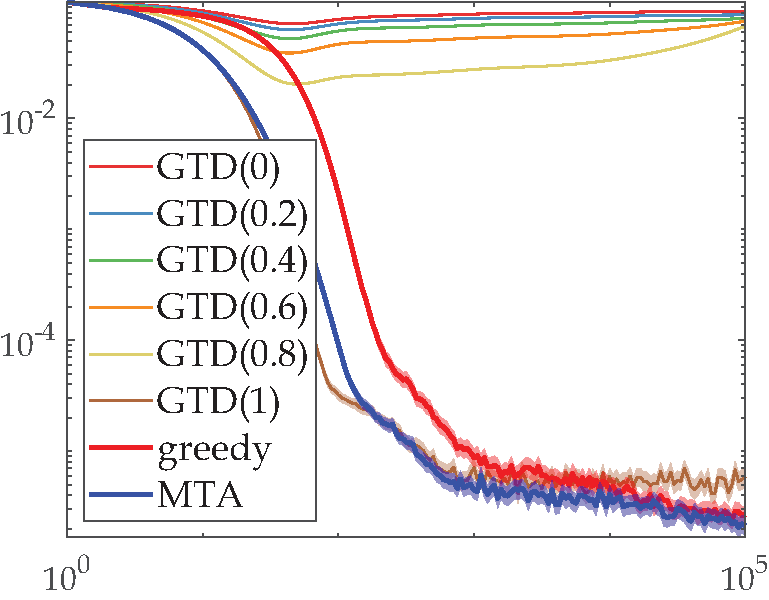
\includegraphics[width=0.4\textwidth]{fig_ringworld_on_1_value.pdf}}
\hfill
\subfloat[$\pi_{l}\!=b_{l}\!=\!0.25$]{
\captionsetup{justification = centering}
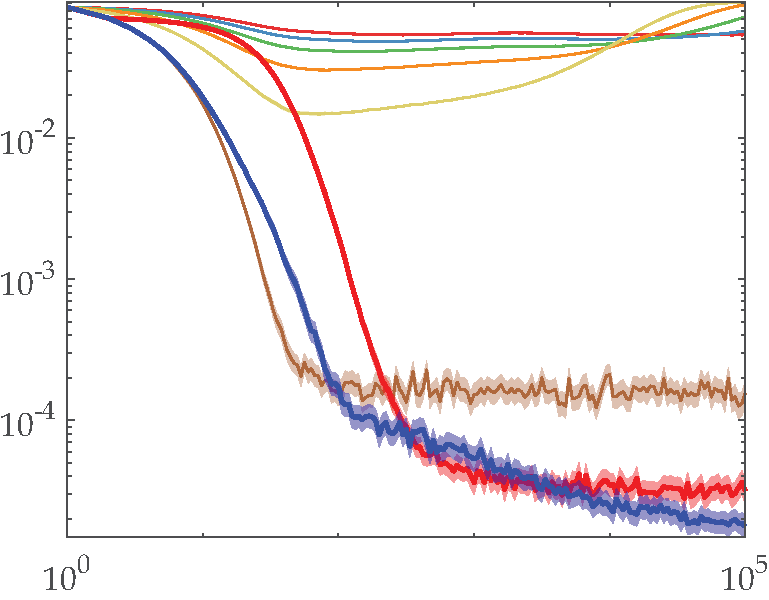
\includegraphics[width=0.4\textwidth]{fig_ringworld_on_2_value.pdf}}
\hfill
\subfloat[$\pi_{l}\!=b_{l}\!=\!0.4$]{
\captionsetup{justification = centering}
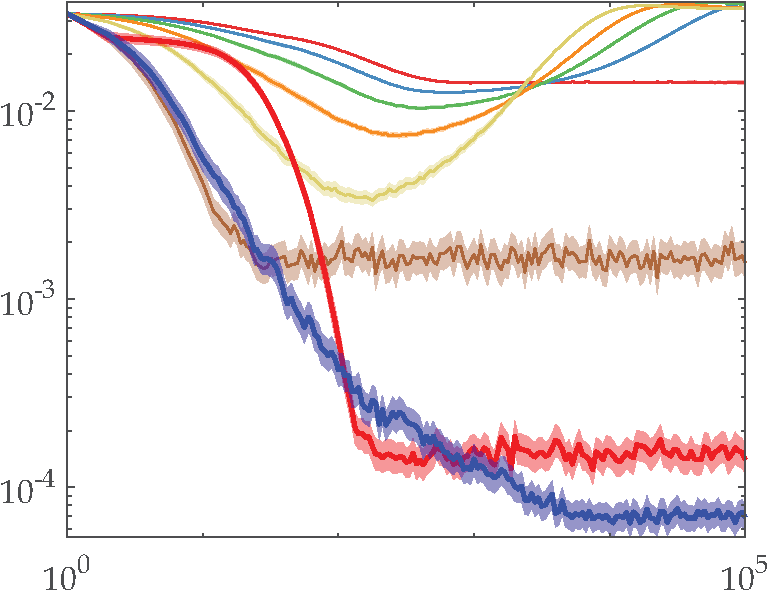
\includegraphics[width=0.4\textwidth]{fig_ringworld_on_3_value.pdf}}

\subfloat[$\pi_{l}\!=\!0.05$, $b_{l}\!=\!0.15$, $\kappa=0.01$]{
\captionsetup{justification = centering}
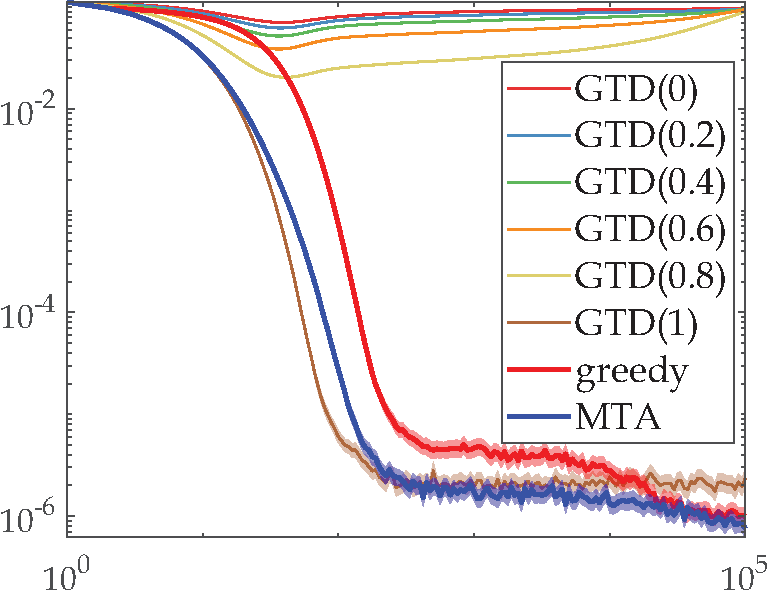
\includegraphics[width=0.4\textwidth]{fig_ringworld_off_1_value.pdf}}
\hfill
\subfloat[$\pi_{l}\!=\!0.25$, $b_{l}\!=\!0.33$, $\kappa=0.01$]{
\captionsetup{justification = centering}
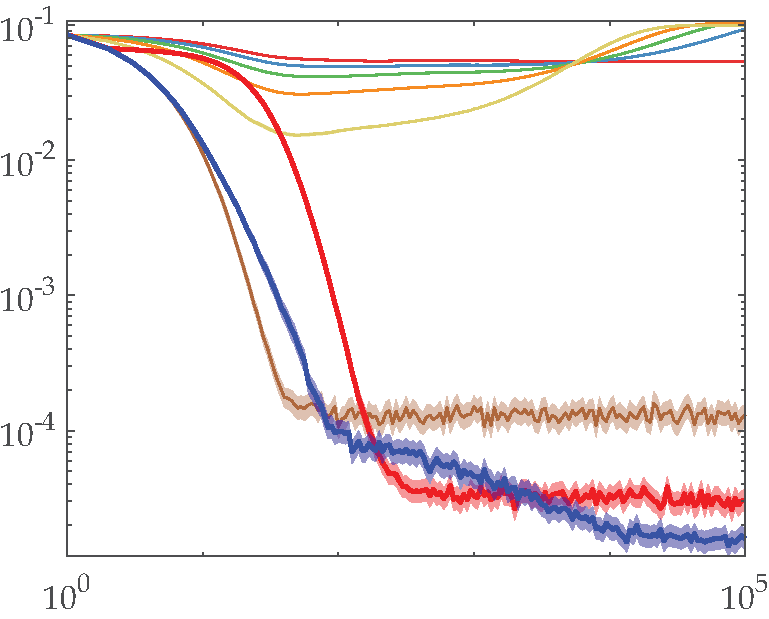
\includegraphics[width=0.4\textwidth]{fig_ringworld_off_2_value.pdf}}
\hfill
\subfloat[$\pi_{l}\!=\!0.4$, $b_{l}\!=\!0.5$, $\kappa=0.01$]{
\captionsetup{justification = centering}
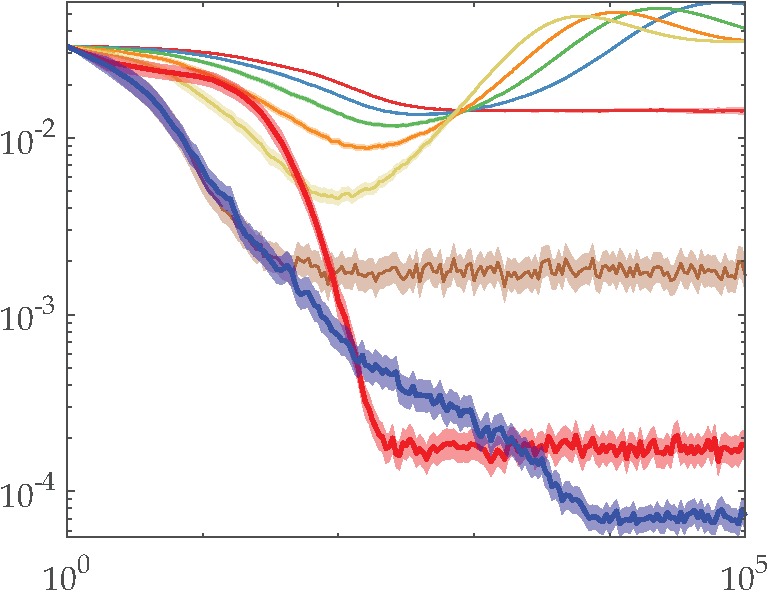
\includegraphics[width=0.4\textwidth]{fig_ringworld_off_3_value.pdf}}

\caption{\small Ringworld tests with $\alpha = \beta = 0.05$ and $\kappa = 0.01$. The x-axes are the number of episodes and the y-axes are errors. We run $100000$ episodes for $160$ independent runs. Baselines of true online GTD($\lambda$) with fixed $\lambda$ values are also provided.}
\label{fig:ringworld_off}
\end{adjustwidth}
\end{figure*}
We also care about MTA's sensitivity to the hyperparameter $\kappa$. If we consider the true online GTD used in $\lambda$-greedy and MTA as a blackbox, then $\lambda$-greedy is parameter free: it adapts $\lambda$ to the minimizer, , whereas MTA does gradient descent controlled by the step-size $\kappa$. In theory, we want the $\kappa$ to be small, in which case the estimates will be stable and good converge is expected. However with limited episodes, we also want $\kappa$ to be not so small \st{} $\Lambda$ can be updated quickly in-time. We can expect a problem-dependent and number-of-episode-dependent range of suitable $\kappa$'s that yield good performance. We present the error curves with different $\kappa$'s in Fig. \ref{fig:ringworld_sensitivity} (a) and the correspondence of final results to $\kappa$'s in Fig. \ref{fig:ringworld_sensitivity} (b).
\begin{figure*}
\centering
\subfloat[$\pi_{l}\!=\!0.05$, $b_{l}\!=\!0.15$]{
\captionsetup{justification = centering}
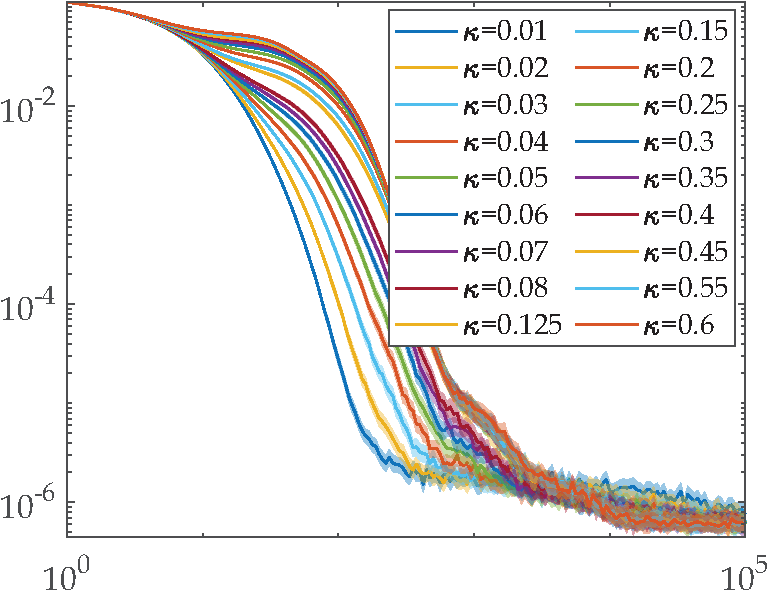
\includegraphics[width=0.45\textwidth]{fig_ringworld_off_1_kappas.pdf}}
\hfill
\subfloat[Sensitivity ($\pi_{l}\!=\!0.05$, $b_{l}\!=\!0.15$)]{
\captionsetup{justification = centering}
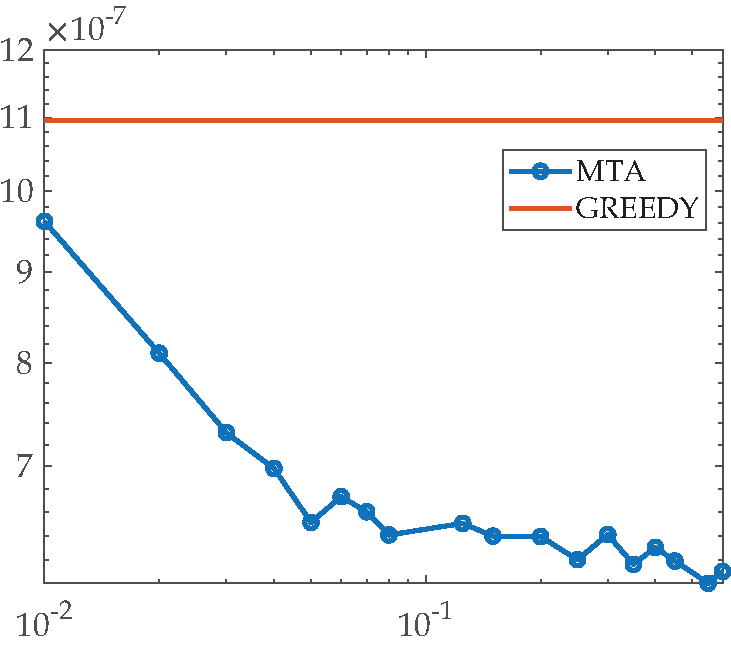
\includegraphics[width=0.45\textwidth]{fig_ringworld_off_1_sensitivity.pdf}}

\caption{\small Sensitivity for $\kappa$ in ringworld. In (b), the x-axis is the values of $\kappa$.}
\label{fig:ringworld_sensitivity}
\end{figure*}
\par
We can see that MTA is relatively robust in terms of the hyperparameter $\kappa$. When the number of episodes is large, we can safely set $\kappa$ to be a small enough value to achieve good convergence.
\subsection{Frozen Lake: Tests with High Variance}
We turn to a high-variance environment, the frozenlake. We craft a uniform policy that takes the actions with equal probabilities and a heuristic policy that has $0.3$ probability for going south or east, $0.2$ for going north or west. We test the on-policy case by setting the behavior and target policies to be the heuristic policy. For off-policy, we use the heuristic as target and the uniform as behavior. The results are presented in Fig. \ref{fig:frozenlake}, alongside the final errors for different $\kappa$'s.
% \footnote{Walk on the surface of a frozen lake to get our frisbee back. We used Gym FrozenLake-v0. Technically, the environment is not a MDP since it is unsolved also with a trajectory length limit. We get the ground truth by running 30 billion simulations using MC.}
\par
We observe that greedy and MTA have similar convergence speed but MTA has better accuracy. The sensitivity curves show that in such a high-variance environment, MTA is robust in terms of $\kappa$. Another reason why MTA performs better than greedy on this environment is that the greedy meta-objective of \cite{white2016greedy} is biased towards MC, and thus biased towards environments in which MC performs better, \ie{} the low-variance environments.
\par


\begin{figure*}
\begin{adjustwidth}{-1in}{-1in}
\centering
\subfloat[On-policy ($\kappa = 0.5$)]{
\captionsetup{justification = centering}
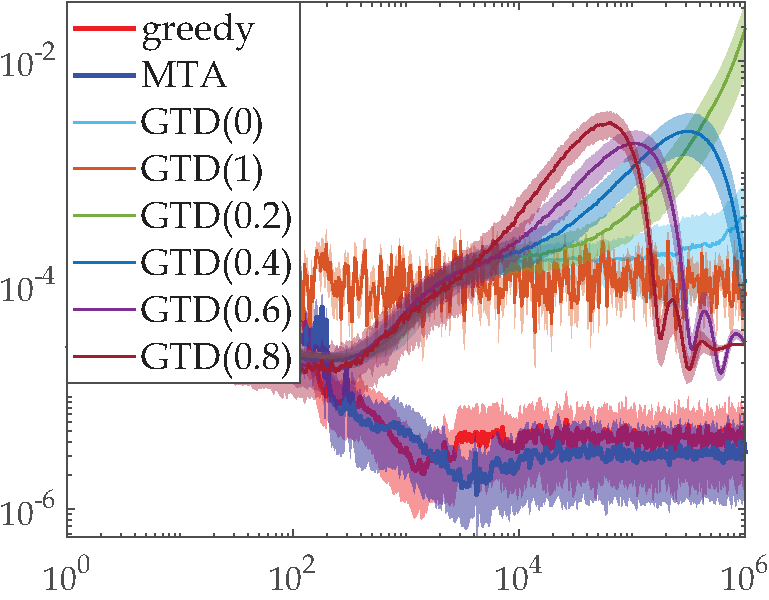
\includegraphics[width=0.31\textwidth]{fig_frozenlake_on_value.pdf}}
\hfill
\subfloat[On-policy sensitivity]{
\captionsetup{justification = centering}
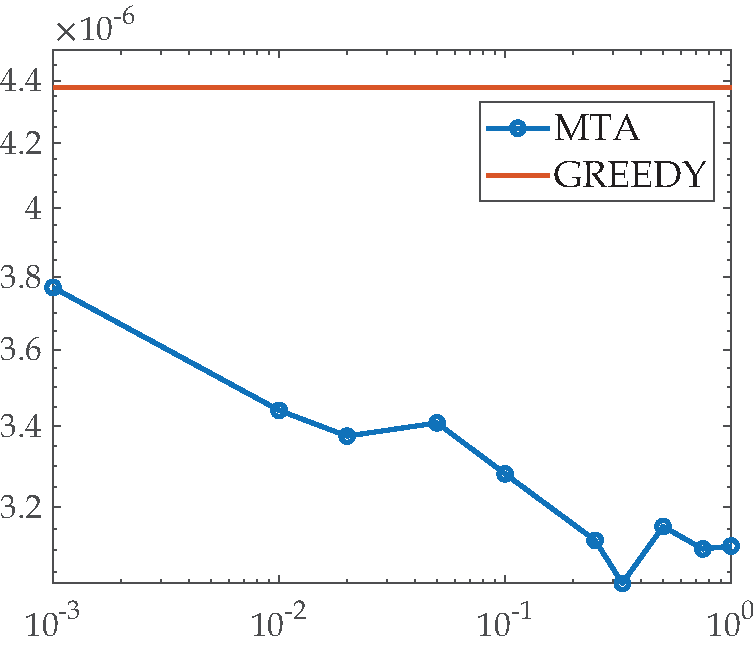
\includegraphics[width=0.31\textwidth]{fig_frozenlake_on_sensitivity.pdf}}
\hfill
\subfloat[Off-policy error with $\kappa = 0.5$]{
\captionsetup{justification = centering}
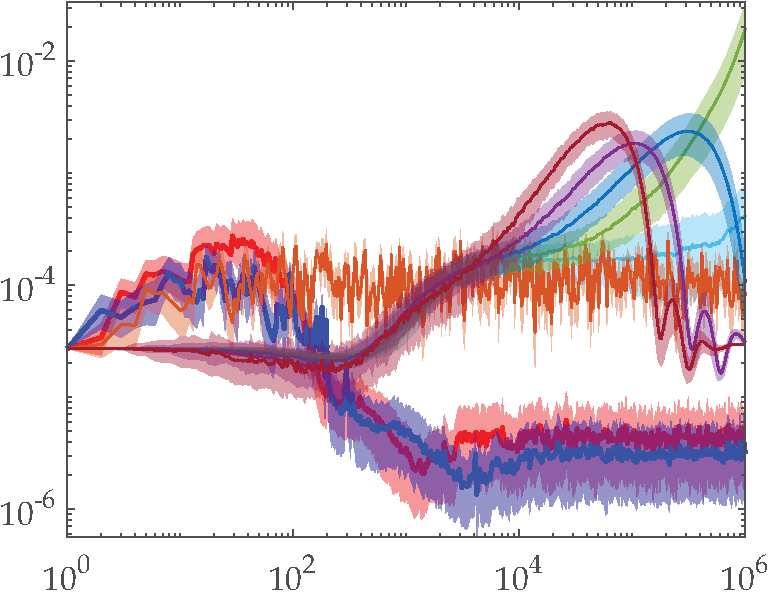
\includegraphics[width=0.31\textwidth]{fig_frozenlake_off_value.pdf}}
\hfill
\subfloat[Off-policy ($\kappa = 0.5$)]{
\captionsetup{justification = centering}
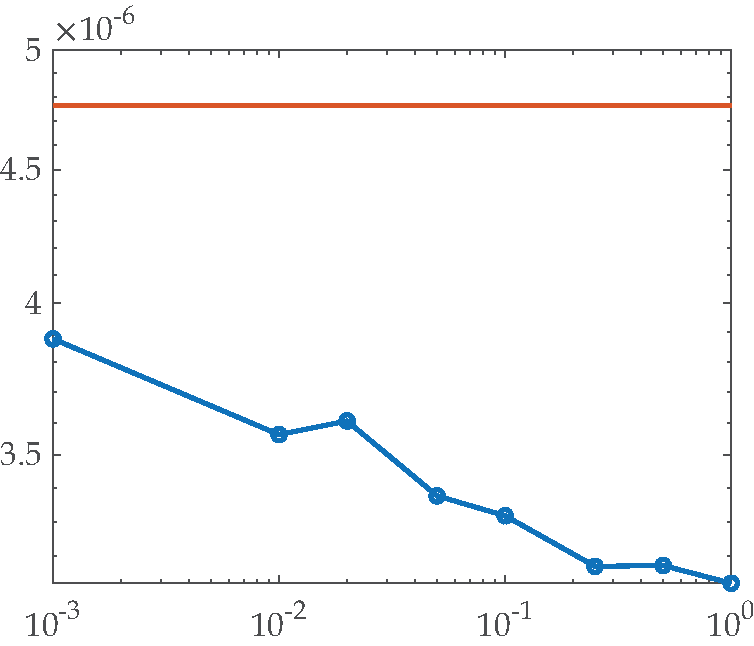
\includegraphics[width=0.31\textwidth]{fig_frozenlake_off_sensitivity.pdf}}
\caption{\small Error curves and sensitivity curves on frozenlake with $\alpha = \beta = 0.05$. Results of MTA on the left are with $\kappa = 0.5$. We run $1000000$ episodes for $160$ independent runs. The sensitivity curves on the right show mean final error with different $\kappa$ values.}
\label{fig:frozenlake}
\end{adjustwidth}
\end{figure*}


\section{Conclusion}
To achieve faster and more accurate policy evaluation using TD($\lambda$), we have derived an algorithm for optimizing the bias-variance tradeoff of the overall target error via meta-learning state dependent $\lambda$'s for TD($\lambda$), with the help of the $\Lambda$-return variance estimation method. The proposed off-policy compatible method MTA, which uses only incremental updates, demonstrates superior empirical performance.

% \section*{Acknowledgements}
% We want to express our sincerest gratitute to Sitao Luan, who has been continuously giving us valuable advice. We also want to thank Prof. Doina Precup for her comments and suggestions. Finally, we are grateful for the computational resources on Compute Canada clusters, supported by Mila.

\bibliographystyle{abbrv}
\bibliography{references}

\newpage
\section*{Appendix}
\subsection{Proof of Proposition \ref{prop:greedy_minimizer}}
\begin{proposition*}
Given the update target $\tilde{G}_t$ of state $s_t$, the minimizer $\lambda_{(t+1)}^*$ of the mean squared target error of the state 
$\tilde{J}(s_t) \equiv \doubleE[{(\tilde{G}_t - \doubleE[G_t])}^2]$ is:
\begin{equation}
\lambda_{(t+1)}^* = \frac{(\doubleE[G_{t+1}] - V(\bm{x}_{t+1}, \bm{w}^{(t)}))^2}{Var[G_{t+1}] + (\doubleE[G_{t+1}] - V(\bm{x}_{t+1}, \bm{w}^{(t)}))^2}
\end{equation}
\end{proposition*}
\begin{proof}
\begin{equation}
\begin{aligned}
J(\lambda^{(t+1)}) & \equiv \doubleE[{(\hat{G}_t - \doubleE[G_t])}^2]\\
& = \doubleE^2[\hat{G}_t - \doubleE[G_t]] + Var[\hat{G}_t - \doubleE[G_t]] && \text{($Var[Z] = \doubleE[Z^2] + \doubleE^2[Z]$)}\\
& = \doubleE^2[\hat{G}_t - G_t] + Var[\hat{G}_t - \doubleE[G_t]] && \text{(both $\doubleE$ are \wrt{} policy)}\\
& \equiv {Bias}^2(\lambda^{(t+1)}) + {Variance}(\lambda^{(t+1)})
\end{aligned}  
\end{equation}

Now we decomposed the objective to the squared bias and the variance. Let us begin by rewriting the bias. Since we have $\bm{x}_t$, $\bm{x}_{t+1}$, $\rho_t$ and $\gamma_{t+1}$,

\begin{equation}
\begin{aligned}
\doubleE[\hat{G}_t] & = \rho_t \doubleE[R_{t+1} + \gamma_{t+1}(1-\lambda^{(t+1)})V(\bm{x}_{t+1}, \bm{w}^{(t)}) + \lambda^{(t+1)} G_{t+1}]\\
& = \rho_t \doubleE[R_{t+1}] + \rho_t \gamma_{t+1} \left((1-\lambda^{(t+1)})V(\bm{x}_{t+1}, \bm{w}^{(t)}) + \lambda^{(t+1)} \doubleE[G_{t+1}]\right)
\end{aligned}
\end{equation}

For convenience, define $err(\bm{w}, \bm{x}_{t+1}) \equiv \doubleE[G_{t+1}] - V(\bm{x}_{t+1}, \bm{w}^{(t)})$ as the difference between the $\lambda = 1$ return and the current approximate value from $\bm{x}_{t+1}$ using weights $\bm{w}^{(t)}$. Using the definition, we can rewrite

\begin{equation}
\doubleE[\hat{G}_t] = \doubleE[G_t] - \rho_t \gamma_{t+1} (1-\lambda^{(t+1)})err(\bm{w}^{(t)}, \bm{x}_{t+1})
\end{equation}

Thus

\begin{equation}
{Bias}^2(\lambda^{(t+1)}) = \doubleE^2[\hat{G}_t - G_t] = \rho_t^2 \gamma_{t+1}^2 (1 - \lambda^{(t+1)})^2 {err}^2(\bm{w}^{(t)}, \bm{x}_{t+1})
\end{equation}

Assuming the noise in the reward $R_{t+1}$ given $\bm{x}_{t}$ and $\bm{x}_{t+1}$ is independent of other dynamics
\begin{equation}
\begin{aligned}
Variance(\lambda^{(t+1)}) & = Var[\rho_t(R_{t+1} + \gamma_{t+1} [(1 - \lambda^{(t+1)})V(\bm{x}_{t+1}, w_v^{(t+1)}) + \lambda^{(t+1)} G_{t+1}])]\\
% & = \rho_t^2 \left(Var[R_{t+1}] + \gamma_{t+1}^2 Var[(1 - \lambda^{(t+1)})V(\bm{x}_{t+1}, w_v^{(t+1)}) + \lambda^{(t+1)} G_{t+1}]\right)\\
& = \rho_t^2Var[R_{t+1}] + \rho_t^2\gamma_{t+1}^2\lambda_{(t+1)}^2 Var[ G_{t+1}]% && \text{$(1 - \lambda^{(t+1)})V(\bm{x}_{t+1}, w_v^{(t+1)})$ has no variance}
\end{aligned}  
\end{equation}

Now we can use the derivations to simplify the objective:

\begin{equation}
\begin{aligned}
\lambda_{(t+1)}^* % & = \argmin_{\lambda_{(t+1)} \in [0, 1]}{J(\lambda_{(t+1)})}\\
& = \argmin_{\lambda_{(t+1)} \in [0, 1]}{{Bias}^2(\lambda_{(t+1)}) + Variance(\lambda_{(t+1)})}\\
% & = \argmin_{\lambda_{(t+1)} \in [0, 1]}{\rho_t^2 \gamma_{t+1}^2 (1 - \lambda^{(t+1)})^2 {err}^2(\bm{w}^{(t)}, \bm{x}_{t+1}) + \rho_t^2Var[R_{t+1}] + \rho_t^2\gamma_{t+1}^2\lambda_{(t+1)}^2 Var[ G_{t+1}]}\\
& = \argmin_{\lambda_{(t+1)} \in [0, 1]}{(1 - \lambda^{(t+1)})^2 {err}^2(\bm{w}^{(t)}, \bm{x}_{t+1}) + \lambda_{(t+1)}^2 Var[G_{t+1}]} = \frac{{err}^2(\bm{w}^{(t)}, \bm{x}_{t+1})}{Var[G_{t+1}] + {err}^2(\bm{w}^{(t)}, \bm{x}_{t+1})}
\end{aligned}
\end{equation}
\end{proof}


\subsection{Proof of Proposition \ref{prop:objective}}
\begin{proposition*}
Given the update target $G_t^\Lambda$ of state $s$, the gradient of the mean squared target error of the state $J \equiv \doubleE[(G_t^\Lambda - \doubleE[G_t])^2]$ \wrt{} $\lambda^{(t+1)}$ is:
\begin{equation}
    \begin{aligned}
    & \nabla_{\lambda^{(t+1)}} J(s_t) = \\
    &\gamma_{t+1}^2 \left[\lambda^{(t+1)} \left[ (V(s_{t+1}) - \doubleE[G_{t+1}^\Lambda])^2 + Var[G_{t+1}^\Lambda] \right] + (\doubleE[G_{t+1}^\Lambda] - V(s_{t+1}))
    (\doubleE[G_{t+1}] - V(s_{t+1}))\right]
    \end{aligned}\nonumber
\end{equation}
And its minimizer is:
\begin{equation}
\begin{aligned}
& \argmin_{\lambda^{(t+1)}}{J(\lambda^{(t+1)})} = \frac{
(V(s_{t+1}) - \doubleE[G_{t+1}^\Lambda])
    (V(s_{t+1}) - \doubleE[G_{t+1}])
}
{(V(s_{t+1}) - \doubleE[G_{t+1}^\Lambda])^2 + Var[G_{t+1}^\Lambda]}
\end{aligned}\nonumber
\end{equation}
\end{proposition*}

\begin{proof}
\begin{equation}
J(\lambda^{(t+1)}) \equiv \doubleE[(G_t^\Lambda - \doubleE[G_t])^2] = \doubleE^2[G_t^\Lambda - G_t] + Var[G_t^\Lambda] \equiv {Bias}^2(\lambda^{(t+1)}) + Variance(\lambda^{(t+1)})
\nonumber
\end{equation}

\begin{equation}
\begin{aligned}
& Variance(\lambda^{(t+1)})\\
& = Var[R_{t+1} + \gamma_{t+1} [(1 - \lambda^{(t+1)})V(s_{t+1}) + \lambda^{(t+1)}G_{t+1}^\Lambda]] && \text{(recursive form)}\\
& = Var[R_{t+1}] + \gamma_{t+1}^2 Var[(1 - \lambda^{(t+1)})V(s_{t+1}) + \lambda^{(t+1)}G_{t+1}^\Lambda]] && \text{($R_{t+1}$ \& $G_{t+1}^\Lambda$ are assumed to be uncorrelated)}\\
& = Var[R_{t+1}] + \gamma_{t+1}^2 \lambda_{(t+1)}^2Var[G_{t+1}^\Lambda] && \text{($(1 - \lambda^{(t+1)})V(s_{t+1})$ not random)}
\end{aligned}
\nonumber
\end{equation}

\begin{equation}
\begin{aligned}
Bias(\lambda^{(t+1)}) & \equiv \doubleE[G_t^\Lambda - G_t]\\
& = \doubleE[R_{t+1} + \gamma_{t+1} [(1 - \lambda^{(t+1)})V(s_{t+1}) + \lambda^{(t+1)}G_{t+1}^\Lambda] - (R_{t+1} + \gamma_{t+1} G_{t+1})] \\
& = \gamma_{t+1} (1 - \lambda^{(t+1)})V(s_{t+1}) + \gamma_{t+1} \lambda^{(t+1)} \doubleE[G_{t+1}^\Lambda] - \gamma_{t+1} \doubleE[G_{t+1}]
\end{aligned}
\nonumber
\end{equation}

\begin{equation}
\begin{aligned}
& \nabla_{\lambda^{(t+1)}} J(\lambda^{(t+1)})\\
& \equiv \bm{\nabla}_{\lambda^{(t+1)}} \left(\doubleE[(G_t^\Lambda - \doubleE[G_t])^2] \right)\\
& = \bm{\nabla}_{\lambda^{(t+1)}} \left(\left(\gamma_{t+1} (1 - \lambda^{(t+1)})V(s_{t+1}) + \gamma_{t+1} \lambda^{(t+1)} \doubleE[G_{t+1}^\Lambda] - \gamma_{t+1} \doubleE[G_{t+1}]\right)^2 + Var[R_{t+1}] + \gamma_{t+1}^2 \lambda_{(t+1)}^2Var[G_{t+1}^\Lambda]\right)\\
& = \gamma_{t+1}^2 \bm{\nabla}_{\lambda^{(t+1)}} \left(((1 - \lambda^{(t+1)})V(s_{t+1}) + \lambda^{(t+1)} \doubleE[G_{t+1}^\Lambda] -  \doubleE[G_{t+1}])^2 + \lambda_{(t+1)}^2Var[G_{t+1}^\Lambda]\right)\\
% & = \gamma_{t+1}^2 \bm{\nabla}_{\lambda^{(t+1)}} [ \lambda_{(t+1)}^2 \left(
% V^2(s_{t+1}) + \doubleE^2[G_{t+1}^\Lambda] - 2J(s_{t+1})\doubleE[G_{t+1}^\Lambda] + Var[G_{t+1}^\Lambda] \right)\\
% & + \gamma_{t+1}^2  \lambda^{(t+1)} \left(
% -2J^2(s_{t+1}) + 2J(s_{t+1})\doubleE[G_{t+1}^\Lambda] + 2J(s_{t+1})\doubleE[G_{t+1}] - 2\doubleE[G_{t+1}^\Lambda]\doubleE[G_{t+1}]
% \right) ]\\
% & = \lambda^{(t+1)} \left[ V^2(s_{t+1}) + \doubleE^2[G_{t+1}^\Lambda] - 2J(s_{t+1})\doubleE[G_{t+1}^\Lambda] + Var[G_{t+1}^\Lambda] \right] + V(s_{t+1})\doubleE[G_{t+1}^\Lambda] + V(s_{t+1})\doubleE[G_{t+1}]
% -V^2(s_{t+1}) - \doubleE[G_{t+1}^\Lambda]\doubleE[G_{t+1}]\\
& = \gamma_{t+1}^2 \left[\lambda^{(t+1)} \left[ (V(s_{t+1}) - \doubleE[G_{t+1}^\Lambda])^2 + Var[G_{t+1}^\Lambda] \right] + V(s_{t+1})(\doubleE[G_{t+1}^\Lambda] + \doubleE[G_{t+1}]) - V^2(s_{t+1}) - \doubleE[G_{t+1}^\Lambda]\doubleE[G_{t+1}]\right]
\end{aligned}
\nonumber
\end{equation}

The minimizer is achieved by setting the gradient to $0$:
\begin{equation}
\begin{aligned}
& \argmin_{\lambda^{(t+1)}}{J(\lambda^{(t+1)})} = \frac{V^2(s_{t+1}) + \doubleE[G_{t+1}^\Lambda]\doubleE[G_{t+1}]-V(s_{t+1})(\doubleE[G_{t+1}^\Lambda] + \doubleE[G_{t+1}])}{(V(s_{t+1}) - \doubleE[G_{t+1}^\Lambda])^2 + Var[G_{t+1}^\Lambda]}
\end{aligned}
\end{equation}
\end{proof}


\subsection{Proof of Theorem \ref{thm:nongreedy}}
\begin{theorem}
Let $s$'s be the states that the agent experiences when rolling out behavior policy $b$ and $\rho_{acc}$ be the cumulative product of importance sampling ratios from the beginning of an episode until state $s$. Gradient descent on the true state objectives corrected by $\rho_{acc}$ is equivalent to stochastic gradient descent on the overall target error for target policy $\pi$. More specifically:
\small
$$\nabla_{\Lambda} J(\bm{G}(\Lambda)) \approx \sum_{s \sim b}{\rho_{acc} \cdot \nabla_{\lambda^{(t+1)}} J(s)}$$
\normalsize
\end{theorem}
\begin{proof}
\begin{equation}
\begin{aligned}
\frac{1}{2} J(\Lambda) = \sum_{s \in \scriptS}{d_\pi(s) \cdot \frac{1}{2} \doubleE[G^\Lambda(s) - v(s)]^2} \equiv \sum_{s \in \scriptS}{d_\pi(s) \cdot \frac{1}{2} J(\lambda(s))}
\end{aligned}\nonumber
\end{equation}

If we take the gradient \wrt{} $\lambda^{(t+1)}$ we can see that:

\begin{equation}
\begin{aligned}
& \nabla_{\Lambda} J(\Lambda)\\
& = \nabla_{\Lambda} \sum_{s \in \scriptS}{d_\pi(s) \cdot J(\lambda^{(t+1)})}\\
& = \nabla_{\Lambda} \sum_{s \in \scriptS}{\sum_{k=0}^{\infty}{\doubleP\{s_0 \to s, k, \pi, s_0 \sim d(s_0) \} J(\lambda(s))}}\\
& \text{$\doubleP\{\cdots\}$ is the prob. of $s_0 \to s$ in exactly $k$ steps, $s_0$ is sampled from the starting distribution $d(s_0)$.}\\
& = \nabla_{\Lambda} \sum_{s \in \scriptS}{\sum_{k=0}^{\infty}{\sum_{\tau}{\doubleP\{s_0 \xrightarrow{\tau} s, k, \pi, s_0 \sim d(s_0) \} J(\lambda(s))}}}\\
& \text{$\tau$ is a possible trajectory sampled from $s_0$ and transitioning to $s$ with exactly $k$ steps}\\
& = \nabla_{\Lambda} \sum_{s \in \scriptS}{\sum_{k=0}^{\infty}{\sum_{\tau}{p(\tau_0, a_0, \tau_1)\pi(a_0|\tau_0) \cdots p(\tau_{k-1}, a_0, s)\pi(a_{k-1}|\tau_{k-1}) J(\lambda(s))}}}\\
& \text{$\tau_i$ is the $i+1$-th state of the trajectory $\tau$ and $p(s, a, s^{'})$ is the probability of $s \xrightarrow{a} s^{'}$ in the MDP}\\
& = \nabla_{\Lambda} \sum_{s \in \scriptS}{\sum_{k=0}^{\infty}{\sum_{\tau}{p(\tau_0, a_0, \tau_1)
\frac{\pi(a_0|\tau_0)}{b(a_0|\tau_0)}
b(a_0|\tau_0)
\cdots p(\tau_{k-1}, a_0, s)
\frac{\pi(a_{k-1}|\tau_{k-1})}{b(a_{k-1}|\tau_{k-1})}
b(a_{k-1}|\tau_{k-1}) J(\lambda(s))}}}\\
& \text{inject importance sampling ratios}\\
\end{aligned}\nonumber
\end{equation}
\begin{equation}
\begin{aligned}
& = \nabla_{\Lambda} \sum_{s \in \scriptS}{\sum_{k=0}^{\infty}{\sum_{\tau}{p(\tau_0, a_0, \tau_1) \rho_{0} b(a_0|\tau_0) \cdots p(\tau_{k-1}, a_0, s) \rho_{k-1} b(a_{k-1}|\tau_{k-1}) J(\lambda(s))}}}\\
& \text{$\rho_{i} \equiv \frac{\pi(a_i | \tau_i)}{b(a_i | \tau_i)}$ is the importance sampling ratio}\\
& = \nabla_{\Lambda} \sum_{s \in \scriptS}{\sum_{k=0}^{\infty}{\sum_{\tau}{\rho_{0:k-1} \cdot p(\tau_0, a_0, \tau_1)  b(a_0|\tau_0) \cdots p(\tau_{k-1}, a_0, s) b(a_{k-1}|\tau_{k-1}) J(\lambda(s))}}}\\
& \text{$\rho_{0:i} \equiv \prod_{v=0}^{i}{\rho_{v}}$ is the importance sampling ratio of the trajectory $\tau$ from $\tau_0$ until $\tau_i$}\\
& = \sum_{s \in \scriptS}{\sum_{k=0}^{\infty}{\sum_{\tau}{\rho_{0:k-1} \cdot p(\tau_0, a_0, \tau_1)  b(a_0|\tau_0) \cdots p(\tau_{k-1}, a_0, s) b(a_{k-1}|\tau_{k-1}) \frac{1}{2} \nabla_{\lambda(s)} J(\lambda(s))}}}\\
& \text{push the gradient inside and $\nabla_{\Lambda}$ becomes $\nabla_{\lambda(s)}$}\\
& \approx \sum_{s \sim b}{\rho_{0:t-1} \cdot \nabla_{\lambda(s)} J(\lambda(s))}\\
& \text{the sums are equivalent to summing over the experiencing states driven by $b$}
\end{aligned}\nonumber
\end{equation}
\end{proof}
\subsection{Experiment Details}
\subsubsection{Feature Engineering}
We used binary features.
\subsubsection{Ground Truths}
We use dynamic programming to solve the ground truth values for computing the error for the ringworld tests. Frozenlake cannot be solved, since it has an episode length limit that destroys its Markov property. We do $30$ billion Monte Carlo simulations to get the ground truth.
\subsubsection{Reproduction of $\lambda$-greedy}
Due to the instability experienced while trying to reproduce the Whites' experiments, we have replaced GTD used in the greedy algorithm with the more stable and robust true online GTD. Also, due to unknown reasons which caused VTD performed extremely unstably, we have replaced the VTD using the direct variance estimation Bellman operator, since they are mathematically equivalent but the latter is more stable and robust empirically. These modifications to the Whites' algorithms are expected only to improve its stability and robustness, without touching the core mechanisms of their algorithm.
\subsubsection{Implementation of MTA}
Due to the instability of the estimates, there could be gradient updates that causes a $\lambda$ value outside the range of $[0, 1]$. In the implementation, whenever we detect such kind of gradient descent step, we simply cancel that operation.

\subsection{Pseudocode of True Online GTD($\Lambda$)}
\begin{algorithm}
\label{alg:true_online_GTD_Lambda}
\caption{True Online GTD($\lambda$) \cite{hasselt2014true}: $\bm{w}^{(t+1)} = togtd(R_{t+1}, \gamma_{t+1},\lambda_{t},\lambda_{t+1},\rho_t)$}
$\delta_t = R_{t+1} + \gamma_{t+1} \bm{x}_{t+1}^T \bm{w}^{(t)} - \bm{x}_{t}^T \bm{w}^{(t)}$;\\
$\bm{z}_t = \rho_t \left[\gamma_t \lambda^{(t)} \bm{z}_{t-1} + \alpha_t (1 - \rho_t \gamma_t \lambda^{(t)} \bm{z}_{t-1}^T\bm{x}_{t}) \bm{x}_{t} \right]$;\\
$\bm{z}_t^\nabla = \rho_t \left[ \gamma_t \lambda^{(t)} \bm{z}_{t-1}^\nabla + \bm{x}_{t} \right]$;\\
$\bm{z}_t^{\bm{h}} = \rho_{t-1} \gamma_t \lambda^{(t)} \bm{z}_{t-1}^{\bm{h}} + \beta_t (1 - \rho_{t-1} \gamma_t \lambda^{(t)} \bm{x}_{t}^T \bm{z}_{t-1}^{\bm{h}})\bm{x}_{t}^T$;\\
$\bm{w}^{(t+1)} = \bm{w}^{(t)} + \delta_t \bm{z}_t + (\bm{w}^{(t)} - \bm{w}^{(t-1)})^T \bm{x}_t(\bm{z}_t - \alpha_t \rho_t \bm{x}_t) - \alpha_t \gamma_{t+1}(1-\lambda^{(t+1)})\bm{h}_t^T \bm{z}_t^\nabla \bm{x}_{t+1}$;\\
$\bm{h}_{t+1} = \bm{h}_{t} + \rho_t \delta_t \bm{z}_t^{\bm{h}} - \beta_t \bm{x}_t^T\bm{h}_{t}\bm{x}_t$;\\
\end{algorithm}
\subsection{On-policy Test Results on Ringworld}
\begin{figure*}
\centering
\begin{adjustwidth}{-1.2in}{-1.2in}
\subfloat[$\pi_{l}\!=b_{l}\!=\!0.05$]{
\captionsetup{justification = centering}
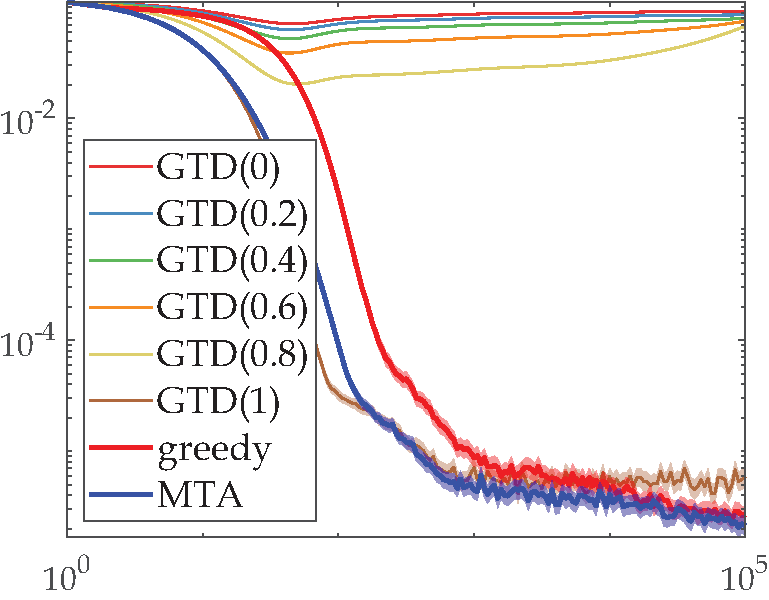
\includegraphics[width=0.45\textwidth]{fig_ringworld_on_1_value.pdf}}
\hfill
\subfloat[$\pi_{l}\!=b_{l}\!=\!0.25$]{
\captionsetup{justification = centering}
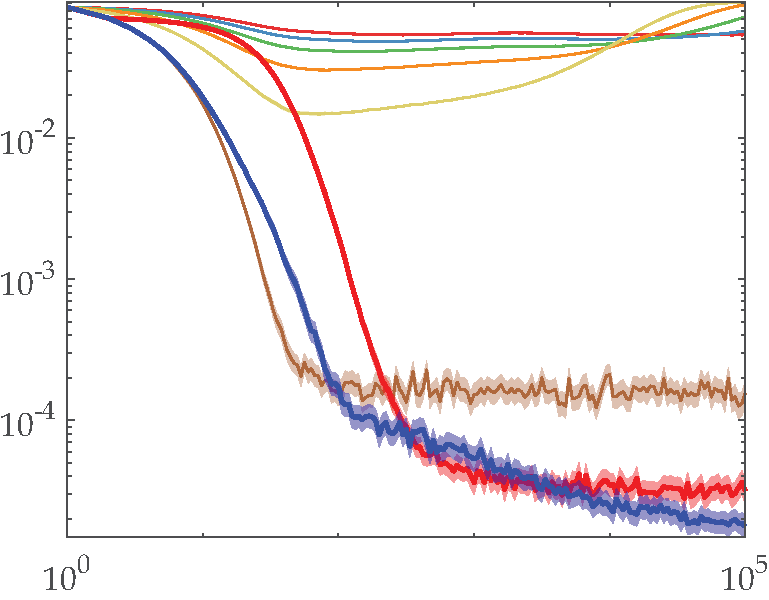
\includegraphics[width=0.45\textwidth]{fig_ringworld_on_2_value.pdf}}
\hfill
\subfloat[$\pi_{l}\!=b_{l}\!=\!0.4$]{
\captionsetup{justification = centering}
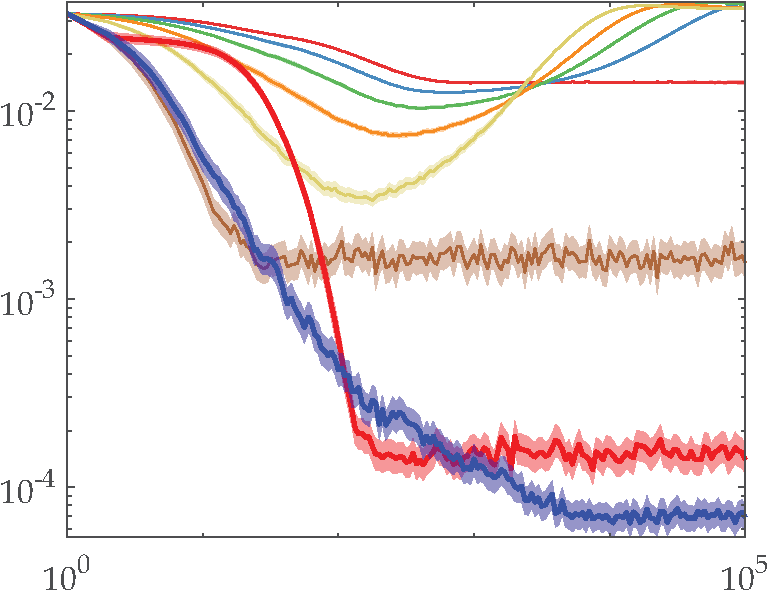
\includegraphics[width=0.45\textwidth]{fig_ringworld_on_3_value.pdf}}
\end{adjustwidth}
\caption{\small On-policy tests on $\gamma = 0.95$ ringworlds.}
\label{fig:ringworld_on}
\end{figure*}

\subsection{$\lambda$ Curves for Tests}
MTA compared to the greedy algorithm: sometimes $\lambda$ converges to zero quickly; Sometimes it bounces and stay relatively high and sometimes it chatters. We think this is a good sign since we are optimizing $\Lambda$ slowly and one $\lambda$ changes along with the changes of the others.
% http://web.mit.edu/jnt/www/Papers/J063-97-bvr-td.pdf
\begin{figure*}
\centering
\begin{adjustwidth}{-1.2in}{-1.2in}
\subfloat[$\pi_{l}\!=\!0.05$, $b_{l}\!=\!0.15$]{
\captionsetup{justification = centering}
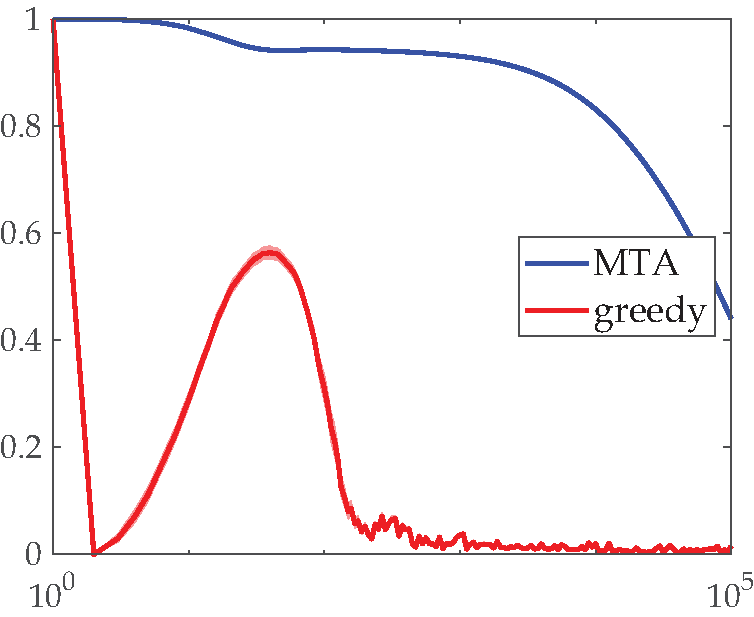
\includegraphics[width=0.45\textwidth]{fig_ringworld_off_1_lambda.pdf}}
\hfill
\subfloat[$\pi_{l}\!=\!0.25$, $b_{l}\!=\!0.33$]{
\captionsetup{justification = centering}
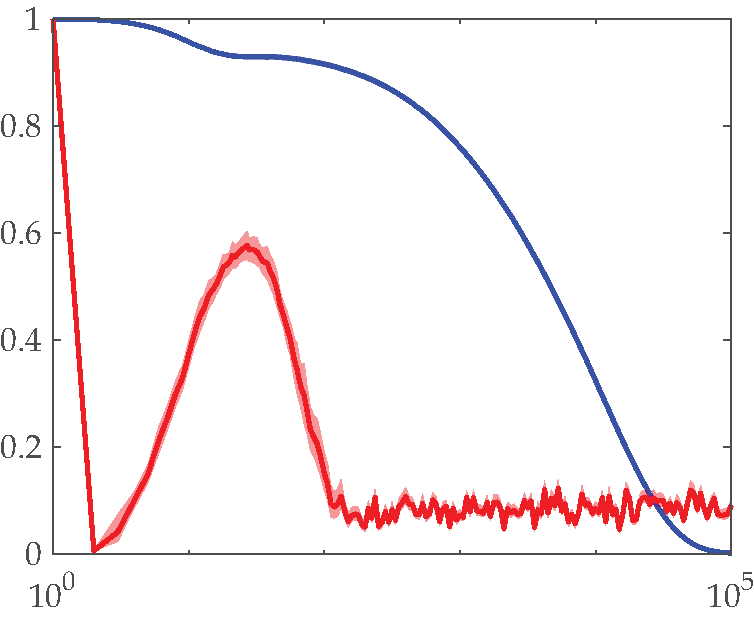
\includegraphics[width=0.45\textwidth]{fig_ringworld_off_2_lambda.pdf}}
\hfill
\subfloat[$\pi_{l}\!=\!0.4$, $b_{l}\!=\!0.5$]{
\captionsetup{justification = centering}
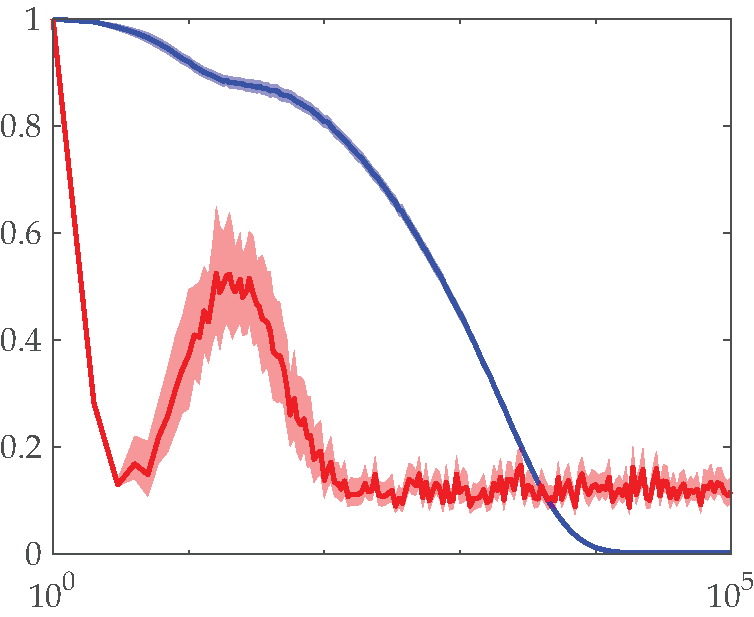
\includegraphics[width=0.45\textwidth]{fig_ringworld_off_3_lambda.pdf}}

\subfloat[$\pi_{l}\!=b_{l}\!=\!0.05$]{
\captionsetup{justification = centering}
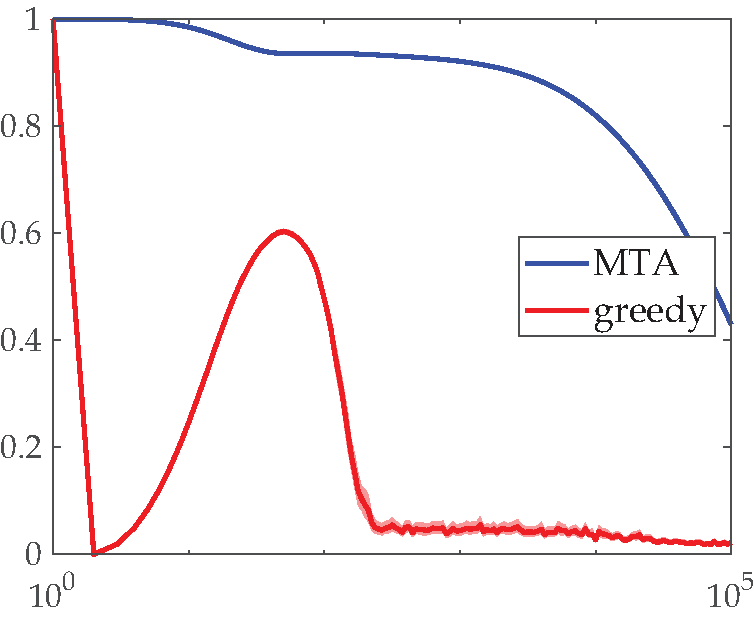
\includegraphics[width=0.45\textwidth]{fig_ringworld_on_1_lambda.pdf}}
\hfill
\subfloat[$\pi_{l}\!=b_{l}\!=\!0.25$]{
\captionsetup{justification = centering}
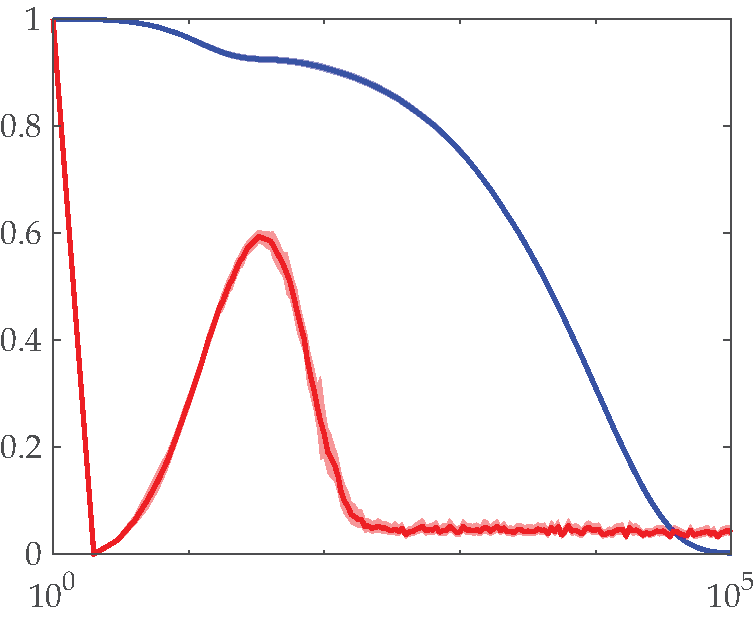
\includegraphics[width=0.45\textwidth]{fig_ringworld_on_2_lambda.pdf}}
\hfill
\subfloat[$\pi_{l}\!=b_{l}\!=\!0.4$]{
\captionsetup{justification = centering}
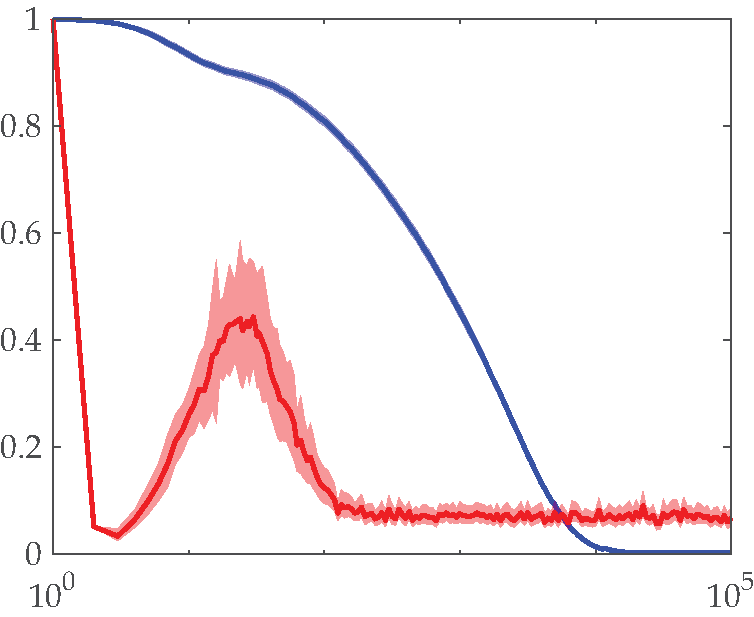
\includegraphics[width=0.45\textwidth]{fig_ringworld_on_3_lambda.pdf}}
\end{adjustwidth}
\caption{\small $\lambda(s_0)$ on $\gamma = 0.95$ ringworlds.}
\label{fig:ringworld_lambda}
\end{figure*}
% http://web.mit.edu/jnt/www/Papers/J063-97-bvr-td.pdf
\end{document}